\subsection{Results}
\footnote{probably want just one Sokoban in the Table;, need Roland to help decide which}


\begin{table}[t]
\footnotesize
  \caption{Performance over granularity levels relative to \tloA{}. Items are significantly different from \tloA{} when marked *$p<0.05$, ** $p <0.01$, *** $p<0.001$; arrows mark the direction of significant differences. Sokoban SFELLA and EEBA use a reward scaling of 0.01.}
  \label{tab:granularity_significance}
\begin{adjustbox}{width=\columnwidth}

\begin{tabular}{>{\raggedright\arraybackslash}p{5em}>{\raggedleft\arraybackslash}p{4em}>{\raggedright\arraybackslash}p{4.5em}rrrr}
\toprule
Environment & RewGranularity & PenGranularity & LIN_SUM & SFLLA1 & EEBA1 & TLO$^A$\\
\midrule
 &  & 0.01 & 1.47*** & 6.61*** & 1.51** & \\

 &  & 1.00 & 1.57** & 4.08*** & 1.46*** & \\

 & \multirow[t]{-3}{4em}{\raggedleft\arraybackslash 0.00} & 100.00 & 1.44*** & 1.39*** & 1.58* & \\
\cmidrule{2-6}
 & 0.01 &  & 1.38*** & 6.47*** & 1.42*** & \\
\cmidrule{2-2}
\cmidrule{4-6}
 & 1.00 &  & 1.46*** & 6.37*** & 1.09*** & \\
\cmidrule{2-2}
\cmidrule{4-6}
\multirow[t]{-6}{5em}{\raggedright\arraybackslash Breakable Bottles} & 100.00 & \multirow[t]{-3}{4.5em}{\raggedright\arraybackslash 0.00} & 1.49** & -40.38*** & -41.39*** & \multirow[t]{-6}{*}{\raggedleft\arraybackslash 1.82}\\
\cmidrule{1-7}
 &  & 0.01 & -0.48*** & 4.02 & 1.50*** & \\

 &  & 1.00 & -0.51*** & 4.64*** & 1.39*** & \\

 & \multirow[t]{-3}{4em}{\raggedleft\arraybackslash 0.00} & 100.00 & -0.45*** & -1.02*** & -1.08*** & \\
\cmidrule{2-6}
 & 0.01 &  & -0.47*** & 3.96 & 0.92*** & \\
\cmidrule{2-2}
\cmidrule{4-6}
 & 1.00 &  & -0.46*** & 3.80 & 1.17*** & \\
\cmidrule{2-2}
\cmidrule{4-6}
\multirow[t]{-6}{5em}{\raggedright\arraybackslash Doors} & 100.00 & \multirow[t]{-3}{4.5em}{\raggedright\arraybackslash 0.00} & -0.38*** & -39.01*** & -41.87*** & \multirow[t]{-6}{*}{\raggedleft\arraybackslash 3.96}\\
\cmidrule{1-7}
 &  & 0.01 & -14.97*** & -10.31*** & -15.01*** & \\

 &  & 1.00 & -14.96*** & -14.90*** & -14.96*** & \\

 & \multirow[t]{-3}{4em}{\raggedleft\arraybackslash 0.00} & 100.00 & -15.05*** & -15.01*** &  & \\
\cmidrule{2-5}
 & 0.01 &  & -15.00*** & -10.83*** & \multirow[t]{-2}{*}{\raggedleft\arraybackslash -14.99***} & \\
\cmidrule{2-2}
\cmidrule{4-6}
 & 1.00 &  & -14.98*** & -7.43*** & -14.86*** & \\
\cmidrule{2-2}
\cmidrule{4-6}
\multirow[t]{-6}{5em}{\raggedright\arraybackslash Sokoban} & 100.00 & \multirow[t]{-3}{4.5em}{\raggedright\arraybackslash 0.00} & -14.96*** & -9.44*** & -10.52*** & \multirow[t]{-6}{*}{\raggedleft\arraybackslash 10.80}\\
\cmidrule{1-7}
 &  & 0.01 & 28.72*** & 27.94*** & 28.73*** & \\

 &  & 1.00 & 28.71*** & 28.77*** & 28.70*** & \\

 & \multirow[t]{-3}{4em}{\raggedleft\arraybackslash 0.00} & 100.00 & 28.77*** & 28.72*** & 28.76*** & \\
\cmidrule{2-6}
 & 0.01 &  & 28.76*** & 27.91*** & 28.73*** & \\
\cmidrule{2-2}
\cmidrule{4-6}
 & 1.00 &  & 28.73*** & 27.79*** & 28.64*** & \\
\cmidrule{2-2}
\cmidrule{4-6}
\multirow[t]{-6}{5em}{\raggedright\arraybackslash Unbreakable Bottles} & 100.00 & \multirow[t]{-3}{4.5em}{\raggedright\arraybackslash 0.00} & 28.74*** & -8.23*** & -13.27*** & \multirow[t]{-6}{*}{\raggedleft\arraybackslash 27.10}\\
\bottomrule
\end{tabular}

\end{adjustbox}
\end{table}


\begin{figure}
  %\centering
  %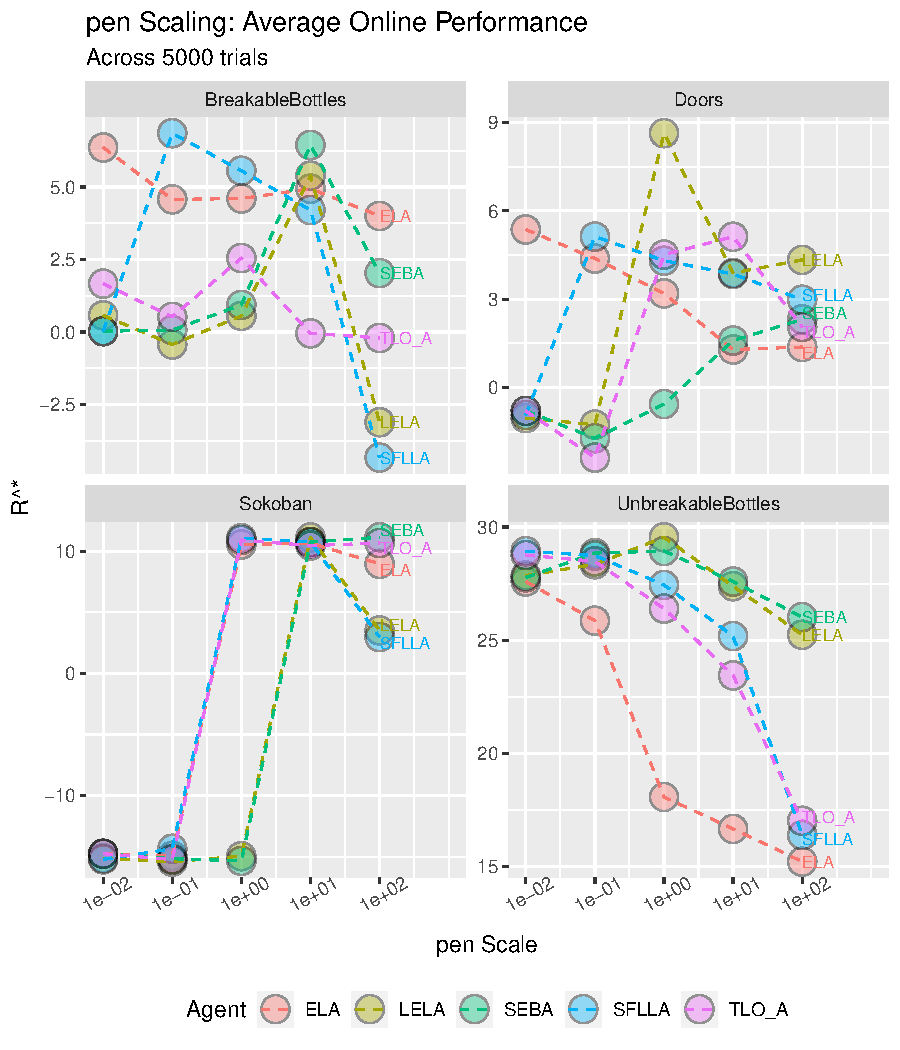
\includegraphics[width=\columnwidth]{output/onlinepen.pdf}
  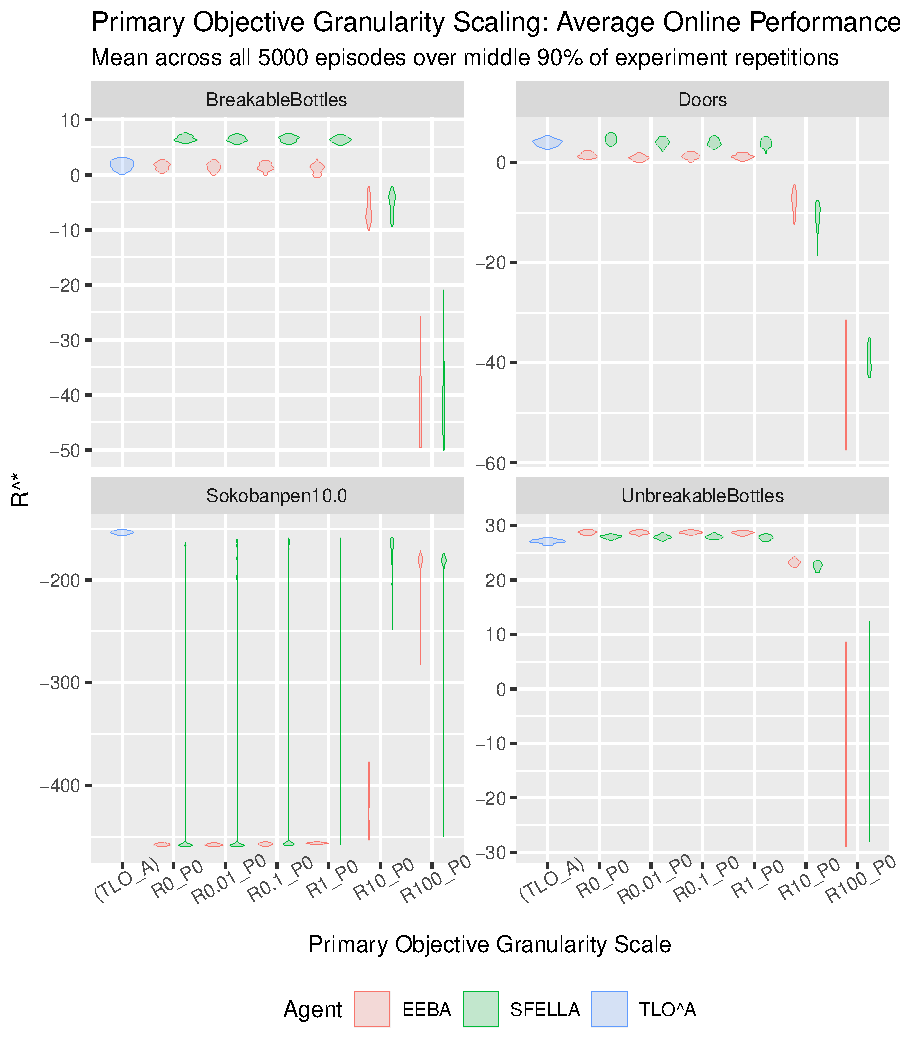
\includegraphics[width=\columnwidth]{output/multirun_n100_pilot_granularity_tunedonline_RewGranularity.pdf}
  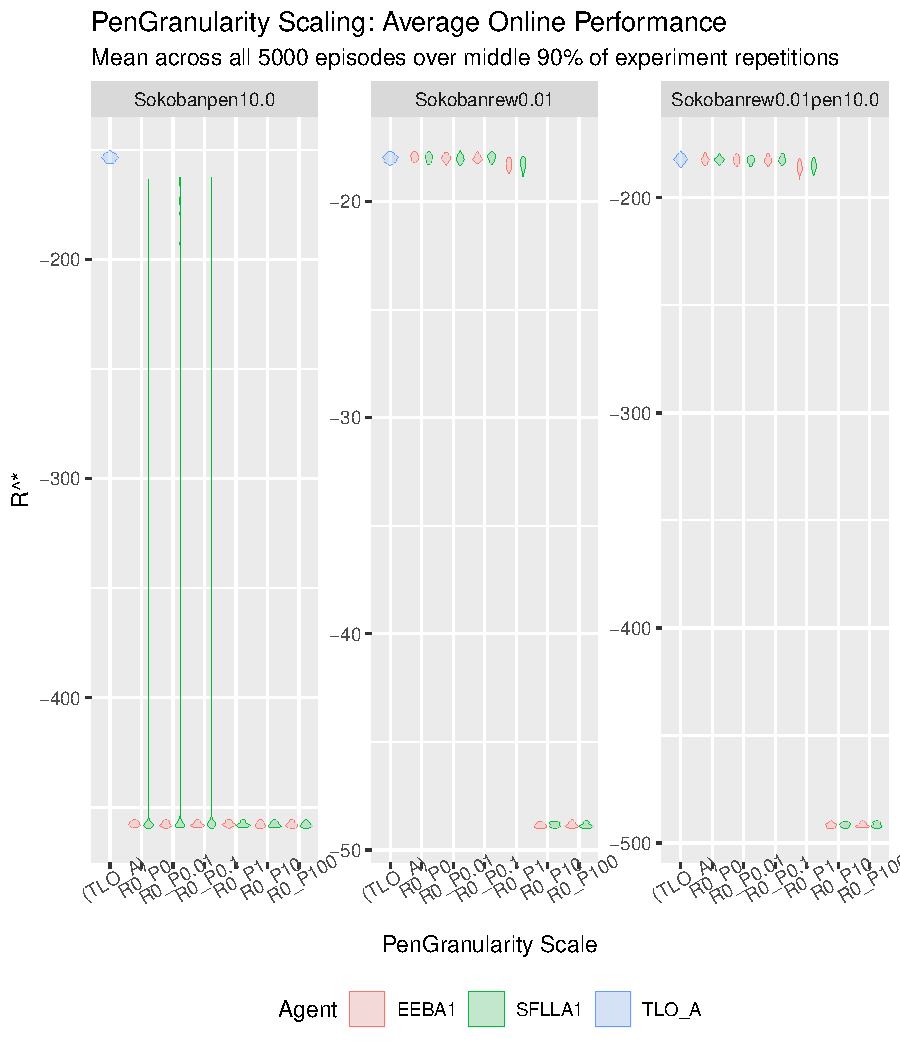
\includegraphics[width=\columnwidth]{output/multirun_n100_pilot_granularity_tunedonline_PenGranularity.pdf}
  \caption{Experiment 3: By creating granularity for our non-linear transform agents, we can simulate similarity with \tloA{}. \tloA{} can be modeled as a non-linear transform with very large granularity, but with a well-tuned offset of the granules. As primary and alignment granularity increases, we become more similar to \tloA{} in that the our agent becomes less sensitive to the changes of rewards. This generally worsens SFELLA performance, particularly in primary objective granularity scaling.
  }
   \label{fig:exp3_main}

 \end{figure}
 
For SFELLA, as expected, \RStar{} performance declined as granularity increased. This was particularly noteable in the BreakableBottles environment where it previously had a clear advantage over \tloA{} (Figure~\ref{fig:exp3_main}). For UnbreakableBottles, performance declined as primary reward granularity increased, but actually marginally improved as penalty granularity was increased.% In the Doors environment, performance declined, from significantly better (??? Table~\ref{tab:granularity_significance}) than \tloA{} to much, much worse. In the Sokoban environment, as in Experiment 1, \tloA{} was the better performer and remained so.

The result confirms that where SFELLA performs well, it does likely so because it avoids `granularity' and is sensitive to changes in reward right across the scale. In contrast, \tloA{} is sometimes insensitive to changes that exceed its threshold. Where it is well tuned, it performs well, or even better, than other algorithms, but when not well-tuned, it performs less well.\footnote{should this be moved to the discussion?}

It can be seen on the plots that performance of SFELLA falls below \tloA{} level on large granularities. Here it is important to note that granularity function has actually two conceptual parameters: the size of granules, and the offset of the granules. In our experiments we changed the size of the granules. At the same time the offset of granules remained implicit and at the zero value. In contrast, for \tloA{} the offset conceptually is same as the threshold value, while the granularity of \tloA{} can be conceptually considered as very large or infinite. For \tloA{} that offset i.e threshold was fine tuned. If we apply similar tuning for SFELLA and fine-tune the offset away from current implicit value of zero then our hypothesis is that the performance of SFELLA will fall to the level of \tloA{} but not lower as the granularity increases. A most reasonable starting point for tuned offset of SFELLA granules would then be equal to the offset i.e threshold that \tloA{} currently has.





